\begin{figure*}[t!]
	\centering

	\subfloat[Known marginal  probabilities.]{
%		\centering
		\scalebox{0.75}{
		\begin{tikzpicture}[>=stealth',shorten >=1pt, on grid,initial/.style={}]
			\node[state, align=center, fill=existential] (T1) {$ 1, 2 $\\$ 0.55 $};
			\node[state, align=center, label={[align=left,right]0:$ 0.85\Pr[Q] + 0.35\Pr[\neg Q] $\\$ =0.55 $}] (T2) [below = 1.6 cm of T1] {$2,1$\\$ 0.55 $};
			\node[state, align=center] (T3) [below left = 1.5 cm and 1.8 cm of T2] {$ 3,0 $\\$ 0.85$};
			\node[state, align=center, fill=terminate] (T4) [below left = 1.5 cm and 1 cm of T3] {$ 4, -1$\\$ 1 $};
			\node[state, align=center] (T5) [below right = 1.5 cm and 1 cm of T3] {$ 4, 0$\\$ 0.7 $};
			\node[state, align=center, fill=terminate] (T6) [below left = 1.5 cm and 1 cm of T5] {$ 5,1 $\\ $0 $};
			\node[state, align=center, fill=terminate] (T7) [below right = 1.5 cm and 1 cm of T5] {$ 5,0 $\\$ 1 $};
			\node[state, align=center] (T8) [below right = 1.5 cm and 1.6 cm of T2] {$ 3,1 $\\$ 0.35 $};
			\node[state, align=center, fill=collision] (T9) [below left = 1.5 cm and 1 cm of T8] {$ 4, 0$\\$ 0.7$};
			\node[state, align=center] (T10) [below right = 1.5 cm and 1 cm of T8] {$ 4, 1$\\$ 0 $};
			\node[state, align=center, fill=terminate] (T11) [below left = 1.5 cm and 1 cm of T10] {$ 5, 2$\\$ 0 $};
			\node[state, align=center, fill=terminate] (T12) [below right = 1.5 cm and 1 cm of T10] {$ 5,1 $\\$ 0 $};
			
			
			
			
			\tikzset{every node/.style={fill=white}}
			\path (T1) edge [right] node {$P$}  (T2);
			\path (T2) edge [left] node {$Q$}  (T3);
			\path (T3) edge [left] node {$R$}  (T4);
			\path (T3) edge [right] node {$\neg R$}  (T5);
			\path (T5) edge [left] node {$S$}  (T6);
			\path (T5) edge [right] node {$\neg S$}  (T7);
			\path (T2) edge [right] node {$\neg Q$}  (T8);
			\path (T8) edge [left] node {$R$}  (T9);
			\path (T8) edge [left] node {$\neg R$}  (T10);
			\path (T10) edge [left] node {$S$}  (T11);
			\path (T10) edge [left] node {$\neg S$}  (T12);
			\end{tikzpicture}
		}
\label{fvgm_fig:example_dp}}
%\hspace*{-0.5cm}
\subfloat[Probabilities computed with a Bayesian network.]
{  
%		\centering
		\scalebox{0.75}{
			\begin{tikzpicture}[>=stealth',shorten >=1pt, on grid,initial/.style={}]
			\node[state, align=center, fill=existential, accepting] (T1) {$ 1, 2 $\\$ 0.65 $};
			\node[state, align=center, accepting, label={[align=left,right]0:$ 0.85\Pr[Q|P] + $ \\ $   0.35\Pr[\neg Q|P] $\\$ =0.65 $}] (T2) [below left = 1.6 cm and 2 cm of T1] {$2,1$\\$ 0.65 $};
			\node[state, align=center] (T3) [below left = 1.5 cm and 1.8 cm of T2] {$ 3,0 $\\$ 0.85$};
			\node[state, align=center, fill=terminate] (T4) [below left = 1.5 cm and 1 cm of T3] {$ 4, -1$\\$ 1 $};
			\node[state, align=center] (T5) [below right = 1.5 cm and 1 cm of T3] {$ 4, 0$\\$ 0.7 $};
			\node[state, align=center, fill=terminate] (T6) [below left = 1.5 cm and 1 cm of T5] {$ 5,1 $\\ $0 $};
			\node[state, align=center, fill=terminate] (T7) [below right = 1.5 cm and 1 cm of T5] {$ 5,0 $\\$ 1 $};
			\node[state, align=center] (T8) [below right = 1.5 cm and 1.6 cm of T2] {$ 3,1 $\\$ 0.35 $};
			\node[state, align=center, fill=collision] (T9) [below left = 1.5 cm and 1 cm of T8] {$ 4, 0$\\$ 0.7$};
			\node[state, align=center] (T10) [below right = 1.5 cm and 1 cm of T8] {$ 4, 1$\\$ 0 $};
			\node[state, align=center, fill=terminate] (T11) [below left = 1.5 cm and 1 cm of T10] {$ 5, 2$\\$ 0 $};
			\node[state, align=center, fill=terminate] (T12) [below right = 1.5 cm and 1 cm of T10] {$ 5,1 $\\$ 0 $};
			
			
			\node[state, align=center, accepting] (T13) [below right = 1.6 and 2 cm of T1] {$2,2$\\$ 0.11 $};
			\node[state, align=center, fill=collision] (T14) [below left = 1.5 and 1 cm of T13] {$3,1$\\$ 0.35 $};
			\node[state, align=center] (T15) [below right = 1.5 and 1 cm of T13] {$3,2$\\$ 0 $};
			\node[state, align=center, fill=collision] (T16) [below left = 1.5 and 1 cm of T15] {$4,1$\\$ 0 $};
			\node[state, align=center] (T17) [below right = 1.5 and 1 cm of T15] {$4,2$\\$ 0 $};
			\node[state, align=center, fill=terminate] (T18) [below left = 1.5 and 1 cm of T17] {$5,3$\\$ 0 $};
			\node[state, align=center, fill=terminate] (T19) [below right = 1.5 and 1 cm of T17] {$5,2$\\$ 0 $};
			
			
			
			\node[state, align=center] (P) [right = 5 cm of T1] {$P$};
			\node[state, align=center] (Q) [right = 2 cm of T15] {$Q$};
			
			
			
			
			
			\tikzset{every node/.style={fill=white}}
			\path (T1) edge [right] node {$P$}  (T2);
			\path (T2) edge [left] node {$Q$}  (T3);
			\path (T3) edge [left] node {$R$}  (T4);
			\path (T3) edge [right] node {$\neg R$}  (T5);
			\path (T5) edge [left] node {$S$}  (T6);
			\path (T5) edge [right] node {$\neg S$}  (T7);
			\path (T2) edge [left] node {$\neg Q$}  (T8);
			\path (T8) edge [left] node {$R$}  (T9);
			\path (T8) edge [left] node {$\neg R$}  (T10);
			\path (T10) edge [left] node {$S$}  (T11);
			\path (T10) edge [left] node {$\neg S$}  (T12);
			\path (T1) edge [right] node {$\neg P$}  (T13);
			\path (T13) edge [right] node {$Q$}  (T14);
			\path (T13) edge [right] node {$\neg Q$}  (T15);
			\path (T15) edge [right] node {$R$}  (T16);
			\path (T15) edge [right] node {$\neg R$}  (T17);
			\path (T17) edge [right] node {$S$}  (T18);
			\path (T17) edge [right] node {$\neg S$}  (T19);
			
			
			
			\path (P) edge [->] node [left=0.1cm] {\parbox{01.2cm}{Bayesian\\network}}(Q);
		\end{tikzpicture}
	}
	\label{fvgm_fig:example_BN}
}

\caption{Search tree representation of {\stochastic} for computing the maximum PPV of the classifier on variables $ \mathbf{B} =  \{P,Q,R,S\} $ with weights $ \{1,1,1,-1\} $ and threshold $ \tau = 2 $ . Each node is labeled by $ (i,\tau') $, where $ i $ is the index of $ \mathbf{B} $ and $ \tau' $ is the residual threshold. The tree is explored using Depth-First Search (DFS) starting with left child. Within a node, the value in the bottom denotes $ \mathsf{dp}(i, \tau') $ that is solved recursively based on sub-problems $ \mathsf{dp}(i+1, \cdot) $ in child nodes. 	Yellow nodes denote \textit{existential} variables and all other nodes are  \textit{random} variables. Additionally, a green node denotes a collision, in which case a previously computed $ \mathsf{dp} $ solution is returned. Leaf nodes (gray) are computed based on terminating conditions in Eq.~\ref{fvgm_eq:dp_terminus}. In Figure~\ref{fvgm_fig:example_BN},  nodes with double circles, such as $ \{(1,2), (2,1), (2,2)\} $,  are enumerated exponentially to compute conditional probabilities from the Bayesian network.}
\label{fvgm_fig:example_tree_exploration}
\end{figure*}	
\subsection{{\stochastic} with Correlated Variables} 
\label{fvgm_sec:dp_with_BN}
In {\stochastic} presented in Section~\ref{fvgm_sec:stochastic_sum_set_sum}, we consider all  Boolean variables to be probabilistically independent. This independence assumption often leads to an \textit{inaccurate estimate} of the probability of positive prediction of the classifier because both sensitive and non-sensitive features can be correlated in practical fairness problems. Therefore, we extend {\stochastic} to include correlations among variables.

We consider a Bayesian network $ \BN = (\graph, \theta) $ to represent correlated variables, where $ G \triangleq (\mathbf{V}, \mathbf{E}) $, $ \mathbf{V} \subseteq \mathbf{B} $, $ \mathbf{E} \subseteq \mathbf{V} \times \mathbf{V}  $, and $ \theta $ is the parameter of the network.  In  $ \BN $, we constrain that there is no conditional probability of choice (i.e., existential and universal) variables as we optimize their assignment in {\stochastic}. Choice variables, however, can impose conditions on chance (i.e., random) variables. In practice, we achieve this by allowing no incoming edge on choice variables while learning $ \BN $ (ref. Section~\ref{fvgm_sec:experiments}).
   	
   	

For a chance variable $ B_i \in \mathbf{V} $, let $ \parent(B_i) $ denote its parents. According to Eq.~\eqref{fvgm_eq:BN},  for an assignment $ \mathbf{u} $ of $ \parent(B_i) $, $ \BN $ ensures $ B_i $ to be independent of other non-descendant variables in $ \mathbf{V} $. Hence, in the recursion of Eq.~\eqref{fvgm_eq:dp_recurse}, we substitute  $ p_i $  with  $ \Pr[B_i = 1| \parent(B_i) = \mathbf{u}] $. In order to explicate the dependence on $ \mathbf{u} $, we denote the expected solution of $ S(\mathbf{B}[i:n], \tau) $ as 
$ \mathsf{dp}(i, \tau, \mathbf{u}) $, which for $ B_i \in \mathbf{V} $ is modified as follows:

\begin{align*}
	\mathsf{dp}(i,  \tau, \mathbf{u}) = & \Pr[B_i = 0| \parent(B_i) = \mathbf{u}] \mathsf{dp}(i+1, \tau, \mathbf{u} \cup \{0\})  \\
	 + & \Pr[B_i = 1| \parent(B_i) = \mathbf{u}]  \mathsf{dp}(i+1, \tau-W_i, \mathbf{u} \cup \{1\}).
\end{align*}

Since $ \mathsf{dp}(i, \tau, \mathbf{u}) $ involves  $ \mathbf{u} $, we initially perform a topological sort of $ \mathbf{V} $ to enumerate the assignment of parents before computing $ \mathsf{dp} $ on the child. Moreover, there are $ 2^{|\parent(B_i)|} $ assignments of $ \parent(B_i) $, and we compute $ \mathsf{dp}(i, \tau, \mathbf{u}) $ for $ \mathbf{u} \in \{0,1\}^{|\parent(B_i)|} $ to incorporate all conditional probabilities into $ \stochastic $.  For this enumeration, we do not store $ \mathsf{dp}(i, \tau, \mathbf{u}) $ in memory. However, for $ B_i \not \in \mathbf{V} $ that does not appear in the network, we instead compute $ \mathsf{dp}(i, \tau) $ and store it in memory as in Section~\ref{fvgm_sec:dp_formulation}, because $ B_i $ is not correlated with other variables.  Lemma~\ref{fvgm_lm:complexity_dp_with_bn} presents the complexity of solving {\stochastic} with correlated variables, wherein unlike Lemma~\ref{fvgm_lemma:complexity_sss}, the  complexity differentiates based on variables in $ \mathbf{V} $ (exponential) and $ \mathbf{B}\setminus \mathbf{V} $ (pseudo-polynomial). 


\begin{lemma}
	\label{fvgm_lm:complexity_dp_with_bn}
	Let $ \mathbf{V} \subseteq \mathbf{B} $ be the set of vertices in the Bayesian network and $ n'' $ be the number of existential and universal variables in $ \mathbf{B} \setminus \mathbf{V} $. Let $$ w'_{\exists} = \sum_{B_i \in \mathbf{B} \setminus \mathbf{V} | Q_i = \exists} \max\{W_i, 0\} \text{ and } w'_{\forall} = \sum_{B_i \in \mathbf{B} \setminus \mathbf{V} | Q_i = \forall} \min\{W_i, 0\}$$ be the sum of considered weights of existential and universal variables, respectively that only appear in $ \mathbf{B} \setminus \mathbf{V} $. To exactly compute {\stochastic} with correlated variables in the dynamic programming approach,  time complexity is $ \mathcal{O}(2^{|\mathbf{V}|} + (n - n'' - |\mathbf{V}|)(\tau + |W_{neg}| - w'_{\exists} - w'_{\forall}) + n'') $ and space complexity is $ \mathcal{O}((n - n'' - |\mathbf{V}|)(\tau + |W_{neg}| - w'_{\exists} - w'_{\forall})) $.
\end{lemma}	


\begin{proof}
	We first separate analysis of space and time complexity for variables in $ \mathbf{V} $ and in $\mathbf{B}\setminus \mathbf{V} $. For each Boolean variable in $ \mathbf{V} $, we enumerate all assignments, which has time complexity of $ 2^{|\mathbf{V}|} $ and there is no space complexity as discussed in Section~\ref{fvgm_sec:dp_with_BN}. 
	
	
	For variables in $\mathbf{B}\setminus \mathbf{V} $, we apply analysis from  Lemma~\ref{fvgm_lemma:complexity_sss}, where we consider $ (n - n'' - |\mathbf{V}|) $ random variables, $ n'' $ existential/universal variables, and residual weights can take at most $ (\tau + |W_{neg}| - w'_{\exists} - w'_{\forall}) $ values. Hence, time complexity is $ \mathcal{O}((n - n'' - |\mathbf{V}|)(\tau + |W_{neg}| - w'_{\exists} - w'_{\forall}) + n'') $, and space complexity is $ \mathcal{O}((n - n'' - |\mathbf{V}|)(\tau + |W_{neg}| - w'_{\exists} - w'_{\forall})) $ 
	
	Combining two cases, overall time complexity is $ \mathcal{O}(2^{|\mathbf{V}|} + (n - n'' - |\mathbf{V}|)(\tau + |W_{neg}| - w'_{\exists} - w'_{\forall}) + n'') $ and space complexity is $ \mathcal{O}((n - n'' - |\mathbf{V}|)(\tau + |W_{neg}| - w'_{\exists} - w'_{\forall})) $. 
\end{proof}

\paragraph{A Heuristic for Faster Computation.} We observe that to encode conditional probabilities, we enumerate all assignments of variables in $ \mathbf{V} $ that are in the Bayesian network. For computing the probability of positive prediction of a linear classifier with correlated features, we consider a heuristic to sort variables in $ \mathbf{B} = \sensitive \cup \nonsensitive $. Let $ \mathbf{V} \subseteq \mathbf{B} $ be the set of vertices in the network and $ \mathbf{V}^c = \mathbf{B} \setminus \mathbf{V} $. In this heuristic, we sort sensitive variables $ \sensitive $ by positioning $ \sensitive \cap \mathbf{V} $ in the beginning followed by $ \sensitive \cap \mathbf{V}^c $. Then we order the variables $ \mathbf{B} $ such that variables in $ \nonsensitive $ precedes those in $ \nonsensitive \cap \mathbf{V} $, and the variables in $ \nonsensitive \cap \mathbf{V}^c $ follows the ones in $ \nonsensitive \cap \mathbf{V} $. This sorting allows us to avoid repetitive enumeration of variables in $ \mathbf{V} \subseteq \mathbf{B} $ as they are placed earlier in $ \mathbf{B} $.

 	 
	\begin{example}
		\normalfont
		We extend Example~\ref{fvgm_example:subset-sum} with a Bayesian Network $ (\graph, \theta) $ with $ \mathbf{V} = \{P, Q\} $ and $ \mathbf{E} = \{(P,Q)\} $. Parameters $ \theta $ imply conditional probabilities $ \Pr[Q|P] = 0.6 $ and $ \Pr[Q|\neg P] = 0.3 $. 	In Figure~\ref{fvgm_fig:example_BN}, we enumerate all  assignment of $ P $ and $ Q $ to  incorporate all conditional probabilities of $ Q $ given $ P $. We, however, observe that the dynamic programming solution in Section~\ref{fvgm_sec:dp_formulation} still prunes search space for variables that do not appear in $ \mathbf{V} $, such as $ \{R, S\} $. Hence following the calculation in Figure~\ref{fvgm_fig:example_BN}, we obtain the maximum probability of positive prediction of the classifier as $ 0.65 $ for $ P = 1 $. The minimum probability of positive prediction (not shown)  is similarly calculated as $ 0.11 $ for $ P = 0 $. 
	\end{example}


	\subsection{Fairness Verification with Computed Probability of Positive Prediction} 
	Given a classifier $\mathcal{M}$, a  distribution $\mathcal{D}$, and a fairness metric $f$, verifying whether a classifier is $\epsilon$-fair for $\epsilon \in [0,1]$ is equivalent to computing $\mathds{1}[f(\mathcal{M}|\mathcal{D})\leq \epsilon]$. We now compute $f(\mathcal{M}|\mathcal{D})$ based on the maximum probability of positive prediction $ \max_{ \mathbf{a}} \Pr[\widehat{Y} =1 | \sensitive = \mathbf{a}] $ and the  minimum probability of positive prediction $ \min_{ \mathbf{a}} \Pr[\widehat{Y} =1 | \sensitive = \mathbf{a}] $ of a classifier.
	
	For measuring fairness metric $ \mathsf{SP} $, we compute the difference $ \max_{ \mathbf{a}} \Pr[\widehat{Y} =1 | \sensitive = \mathbf{a}]  - \min_{ \mathbf{a}} \Pr[\widehat{Y} =1 | \sensitive = \mathbf{a}] $. We, however, deploy {\fvgm} twice while measuring $ \mathsf{EO} $, one for the distribution $ \mathcal{D} $ conditioned on $ Y = 1  $ and another for $ Y = 0 $. In each case, we compute $ \max_{ \mathbf{a}} \Pr[\widehat{Y} =1 | \sensitive = \mathbf{a}, Y = y ]  - \min_{ \mathbf{a}} \Pr[\widehat{Y} =1 | \sensitive = \mathbf{a}, Y = y ] $ for $ y \in \{0,1\} $ and take the  maximum difference as the value of $ \mathsf{EO} $. For measuring causal metric $ \mathsf{PCF} $, we compute  $ \max_{ \mathbf{a}} \Pr[\widehat{Y} =1 | \sensitive = \mathbf{a}, \mathbf{Z}] $ and  $ \min_{ \mathbf{a}} \Pr[\widehat{Y} =1, \mathbf{Z}| \sensitive = \mathbf{a} , \mathbf{Z}] $ conditioned on mediator features $ \mathbf{Z} $ and take their difference. 	To measure disparate impact $ \mathsf{DI} $, we compute the ratio $ \max_{ \mathbf{a}} \Pr[\widehat{Y} =1 | \sensitive = \mathbf{a}] / \min_{ \mathbf{a}} \Pr[\widehat{Y} =1 | \sensitive = \mathbf{a}] $. In contrast to other fairness metrics, $ \mathsf{DI} $ closer to 1 indicates higher fairness level. Thus, we verify whether a classifier achieves $(1 - \epsilon)$-$ \mathsf{DI} $ by checking $ \mathds{1}[f_{\mathsf{DI}}(\alg| \mathcal{D}) \ge 1 - \epsilon] $.
	
	
	
	\subsection{Extension to Practical Settings}\label{fvgm_sec:practical}
	For verifying linear classifiers with real-valued features and coefficients, we preprocess them so that {\fvgm} can be invoked. Let $ X \in \mathbb{R} $ be a continuous real-valued feature with coefficient $ W \in \mathbb{R} $ in the classifier. We discretize $ X $ to a set $ \mathbf{B} $ of $ k $ Boolean variables using binning-based discretization and assign a Boolean variable to each bin. Hence, $ B_i \in \mathbf{B} $ becomes $ 1 $, when $ X $ belongs to the $ i^\text{th} $ bin. Let $ \mu_i $ denote the mean of feature-values within $ i^\text{th} $ bin. We then set the coefficient of $ B_i $ as $ \mu_iW $. By the law of large numbers, $ X \approx \sum_i \mu_iB_i $ for infinitely many bins~\cite{grimmett2020probability}. Finally, we multiply the coefficients of discretized variables by $ l \in \mathbb{N} \setminus \{0\} $ and round to an integer. The accuracy of the preprocessing step relies on the number of bins $ k $ and the multiplier $ l $. Therefore, we empirically fine-tune both $ k $ and $ l $ by comparing  the processed classifier with the initial classifier on a validation dataset.
\begin{comment}
	\begin{figure}
		\centering
		\subfloat[Exploration tree of stochastic sub-set sum problem.]{	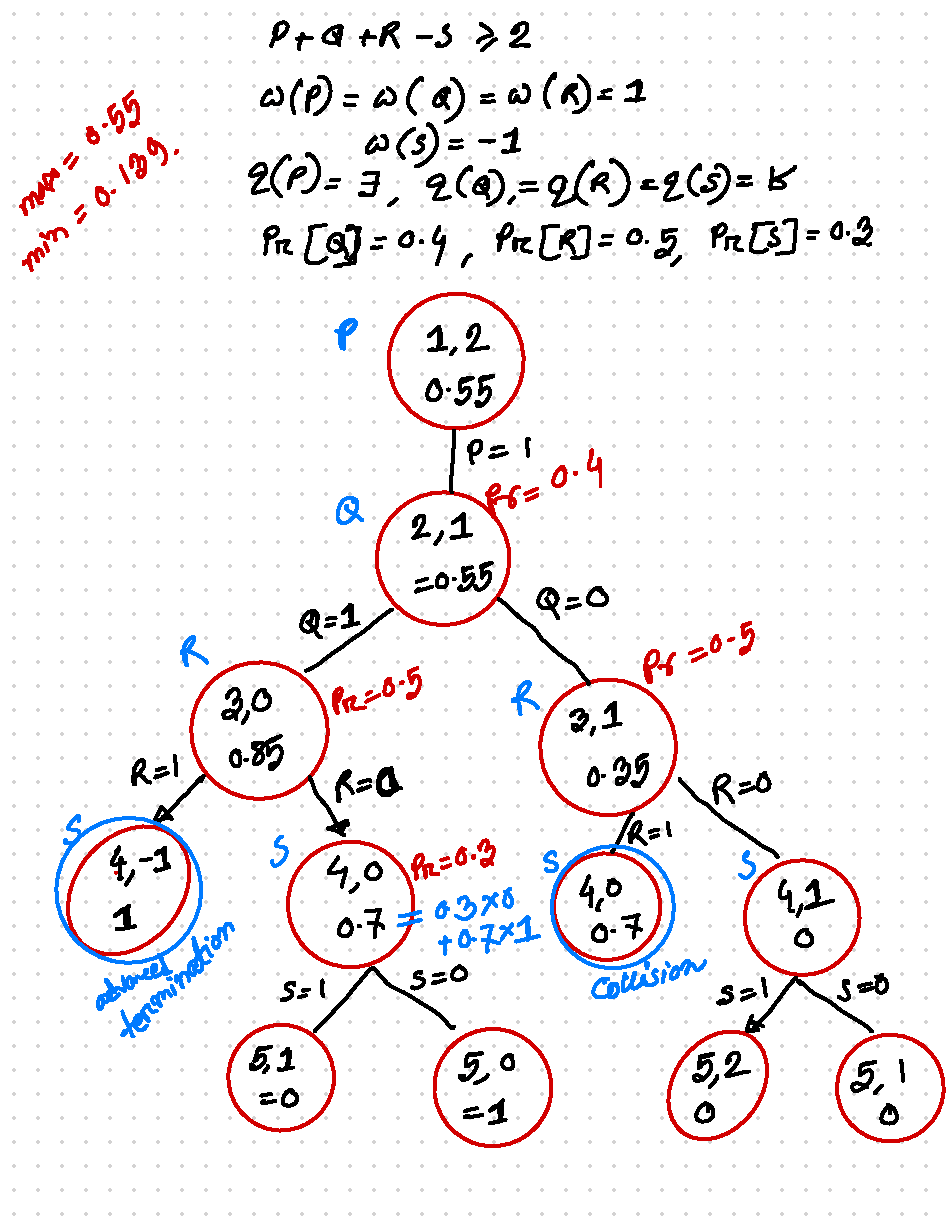
\includegraphics[scale=0.3]{figures/exploration_tree_DP}\label{fvgm_fig:example_dp}}
		\subfloat[Bayesian network]{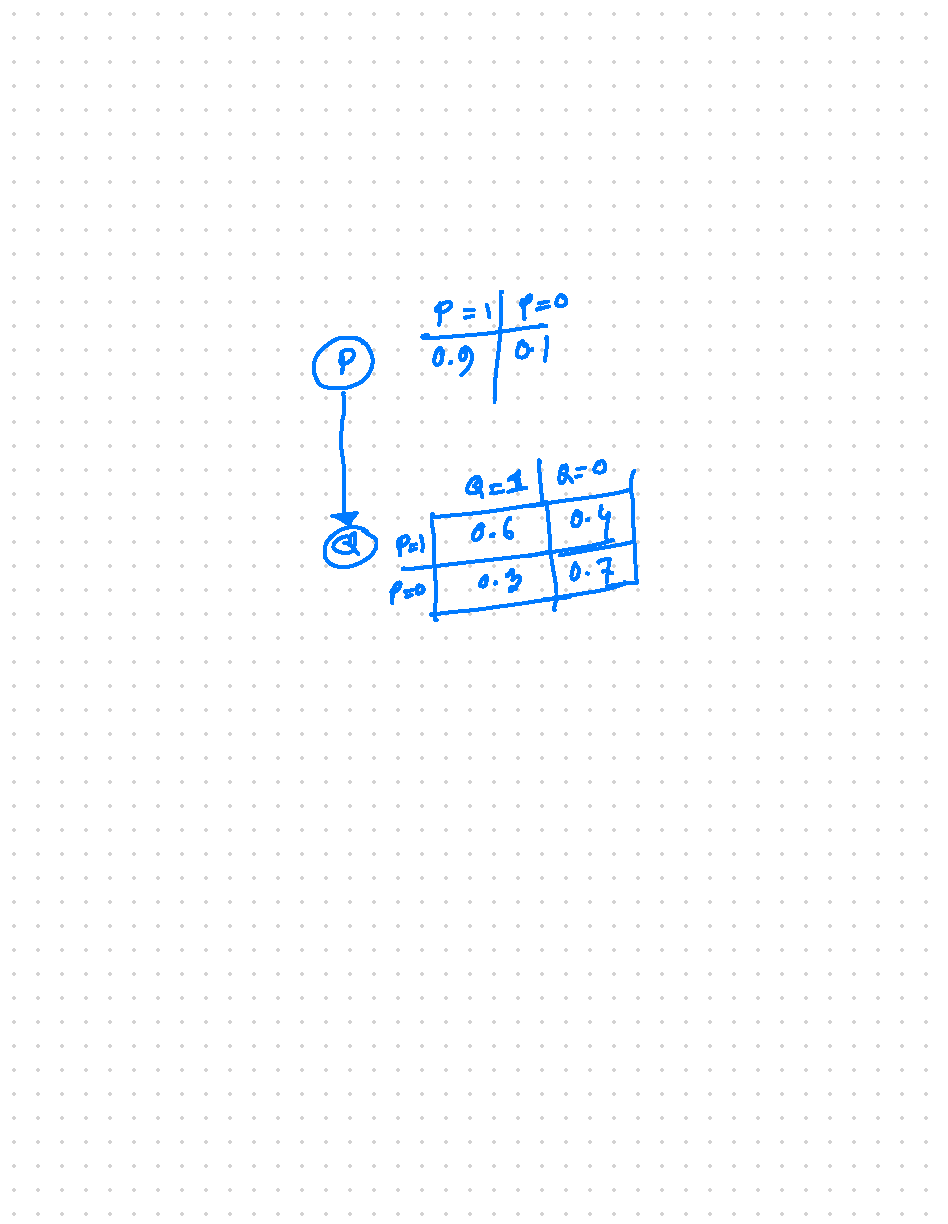
\includegraphics[scale=.4]{figures/example_BN}\label{fvgm_fig:example_BN}}
		\subfloat[Exploration tree of stochastic sub-set sum problem with Bayesian network]{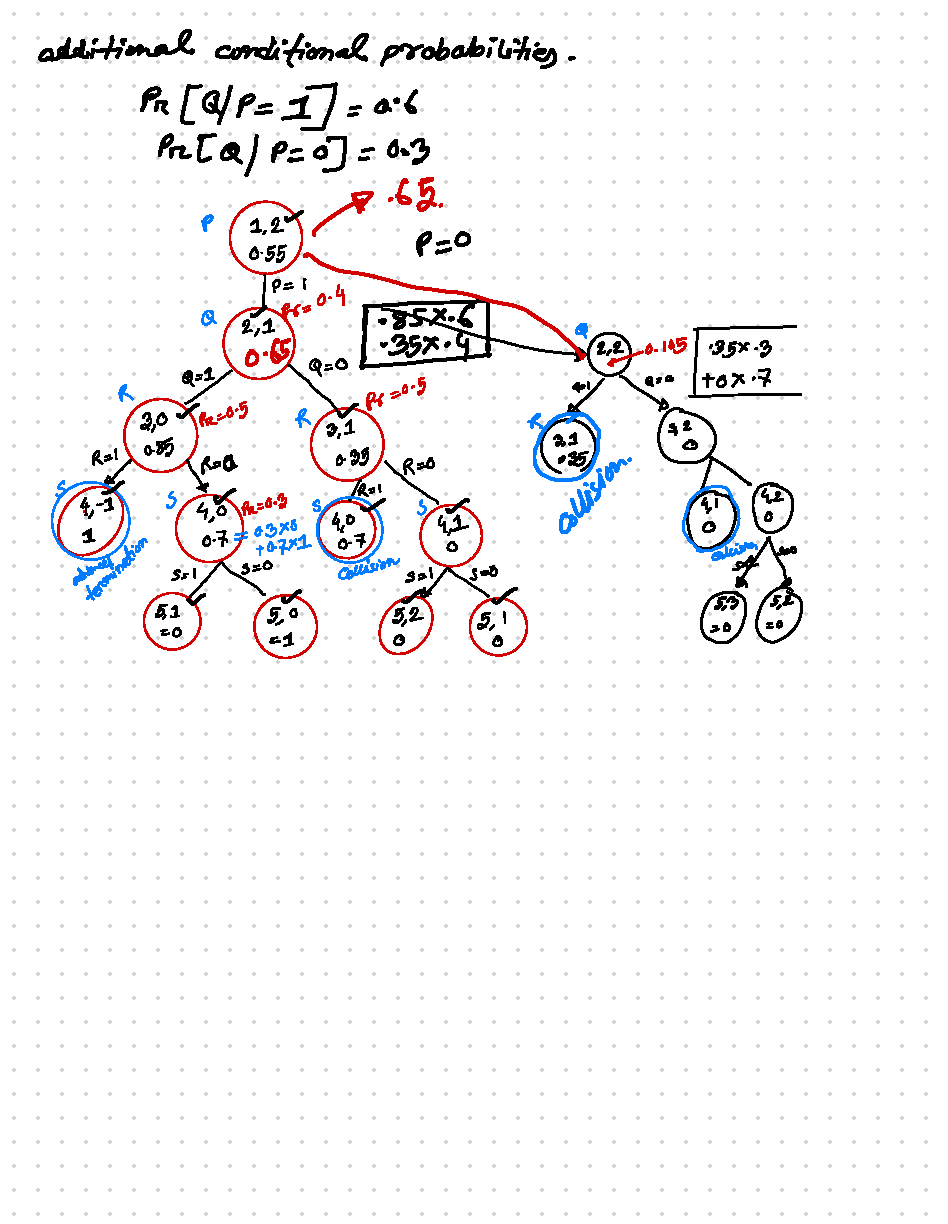
\includegraphics[scale=.4]{figures/exploration_tree_DP_BN}	\label{fvgm_fig:example_dp_BN}
		}
		
	\end{figure}
\end{comment}


